\chapter{Diseño e implementación}\label{cap.implementacion}
\section{Introducción}

Este capítulo está dedicado a la profundización en la constitución del propio simulador así como sus funcionalidades, diseño, modo de uso y estructura. La finalidad del mismo es la de plasmar una visión que englobe todos los aspectos característicos del simulador, desde su concepción y desarrollo hasta su alcance y utilidad.

\section{Visión general del simulador}

Este simulador ha sido desarrollado en su totalidad con la plataforma de desarrollo Matlab, implementando y utilizando exclusivamente \textit{scripts}, funciones, objetos y \textit{frameworks} de dicha plataforma.

Este software ha sido concebido como código libre, por lo que está disponible para su consulta, uso y modificación para todo el mundo a través de la plataforma GitHub, protegido bajo una licencia GNU v3.0, al igual que se encuentra \textit{QuaDRiGa}.

Remarcar también que se ha apostado por una estructura que no modifique en nada el código original de \textit{QuaDRiGa}, por lo que se trata de una implementación totalmente independiente, lo que ofrece como principal ventaja la escalabilidad del mismo y la compatibilidad entre ambos programas en futuras actualizaciones.

La filosofía de diseño del simulador ha sido la de ofrecer al usuario un método accesible e intuitivo de acceder a las simulaciones de \textit{QuaDRiGa} permitiendo flexibilidad en las opciones de entrada, así como un post-procesado de las salidas del generador de canal que permitan al usuario entender qué es lo que está sucediendo en su simulación y el comportamiento de la misma. De este modo, se pretende ahorrar el periodo de documentación sobre la utilización de \textit{QuaDRiGa}, que para adquirir unas nociones de uso avanzado se han dedicado 100 horas en el trascurso de este proyecto, como se señalaba en al Tabla \ref{tab:horas}.

Por ello, este simulador es completamente utilizable sin línea de comandos como sucede en la mayoría de simuladores y software escritos en Matlab. Sin embargo, para extraer datos avanzados de la simulación, como valores numéricos de los distintos parámetros que se obtienen de salida, sí que es necesario trabajar en línea de comandos una vez completa la simulación, puesto que el desarrollo del simulador se ha centrado en su valoración visual a través de herramientas como gráficas.

En primer lugar, se comenzará por detallar los requisitos de sistema que se precisan para su ejecución, como muestra la siguiente sub-sección. Acto seguido, se procederá a mostrar sus características de una forma cualitativa, seguido de una lista de mejoras con respecto al software original -\textit{QuaDRiGa}- y, por último, una descripción de su modo de uso y su correcto funcionamiento.

\subsection{Requisitos de ejecución}

Aunque este software no ha sido probado en una amplia variedad de equipos de distintas plataformas, gracias a Matlab, se puede asegurar una compatibilidad fiable en la mayoría de equipos que sean capaces de ejecutar dicha plataforma de desarrollo.

Sin embargo, la capacidad de cómputo que exigen ciertos cálculos que se llevan a cabo durante las simulaciones de \textit{QuaDRiGa}, así como funcionalidades adicionales que se han implementado posteriormente, hacen que los requisitos para ejecutar el simulador resulten más restrictivos que los originales de \textit{QuaDRiGa}. En concreto, en la Tabla \ref{tab:espec_simulador} se puede encontrar los requisitos que se han estimado tras una fase de prueba en el que se ha medido el rendimiento y los recursos que el simulador ha necesitado durante su ejecución:

\begin{table}[h!]
\centering
\caption{Requisitos mínimos del simulador para una compatibilidad total}
\label{tab:espec_simulador}
\begin{tabular}{c|c}
\textbf{Característica} & \textbf{Requisito mínimo} \\ \hline
Versión de Matlab       & R2017a             \\
Toolbox                 & App Designer                   \\
Memoria (RAM)           & 1,5 GB                      \\
Procesador              & 1 GHz un solo núcleo      \\
Almacenamiento          & 80 MB                     \\
Sistema operativo       & Windows, Mac OS   
\end{tabular}
\end{table}

Como se puede observar, si se compara con las especificaciones de \textit{QuaDRiGa} que aparecían en la Tabla \ref{tab:espec_quadriga}, los requisitos han cambiado volviéndose algo más exigentes. Este cambio está justificado debido al Framework utilizado para implementar la interfaz gráfica, \textit{App Designer}, que viene incluido solamente en versiones de Matlab R2017a y superiores. Del mismo se hablará en futuras secciones.

Además, cierto intercambio de instancias entre clases y funciones se realiza a través del almacenamiento de disco duro, por lo que se requiere de un mínimo mayor de capacidad de almacenamiento con la finalidad de permitir esta transacción de datos. 

Puesto que el simulador no es compatible con Octave, se ha perdido la compatibilidad con Linux.

Por otro lado, cabe destacar que estos son los requisitos para una compatibilidad máxima, especialmente con la interfaz gráfica. Sin embargo, es posible ejecutar una versión minimalista disponible en GitHub que solamente requiere la inserción manual de los parámetros de entrada a partir de la creación de variables a través de \textit{script} o línea de comandos. Para esta versión, los requisitos son los mostrados en la Tabla \ref{tab:espec_simulador_minimalista}:

\begin{table}[h!]
\centering
\caption{Requisitos mínimos del simulador para su versión minimalista sin GUI}
\label{tab:espec_simulador_minimalista}
\begin{tabular}{c|c}
\textbf{Característica} & \textbf{Requisito mínimo} \\ \hline
Versión de Matlab       & R2011a             \\
Toolbox                 & Ninguno                  \\
Memoria (RAM)           & 2 GB disponibles                     \\
Procesador              & 1 GHz un solo núcleo      \\
Almacenamiento          & 80 MB                     \\
Sistema operativo       & Windows, Mac OS   
\end{tabular}
\end{table}

Básicamente, los requisitos de esta versión son los mismos que los de \textit{QuaDRiGa} con la salvedad de la necesidad de un mayor espacio de almacenamiento justificado anteriormente, un incremento de memoria RAM debido a la gran cantidad de datos que se almacenarán en la memoria y la pérdida de la compatibilidad con Octave debido a que el desarrollo ha sido exclusivo para Matlab sin tener en cuenta ninguna otra plataforma de desarrollo o de ejecución.

\subsection{Características}

Aunque el simulador esté basado en \textit{QUaDRiGa} para la generación de sus coeficientes de canal, las características con respecto a su base cambian sustancialmente, ya sea por funcionalidades descartadas en el desarrollo, o bien, por nuevas implementaciones añadidas:

\begin{itemize}
    \item Permite la creación de dos tipos de capas de red, una para macro-celdas y otra para micro-celdas, con hasta 37 estaciones base cada una y sin límite de receptores.
    \item Las características de modelado del entorno vienen establecidas de acuerdo a la normativa de 3GPP TR 38.901, que incluye simulaciones con frecuencias en un rango entre 500 MHz y 100 GHz, con una reutilización unitaria.
    \item Diferenciación de segmentos de visión directa y sin visión directa. La probabilidad de los mismos está determinada por el usuario.
    \item Los terminales móviles se encuentran en movimiento. Cuentan con interfaz dual, una a la frecuencia de las macro-celdas y otra a la de las micro-celdas. Ambas capas de simulación son capaces de compartir los mismos usuarios.
    \item La cobertura de las celdas se encuentran modeladas por una antena omnidireccional en el centro de las mismas a modo de simplificación.
    \item Planificación geométrica de las capas de simulación. Una vez establecido el número de celdas, éstas se distribuyen homogéneamente a través de todo el escenario según la distancia de separación entre ellas que se especifique.
    \item Integra evolución de la señal teniendo en cuenta efectos de pequeña y de gran escala.
    \item Por simplificación de implementación y de costes computacionales, los enlaces son de tipo SISO.
    \item Interfaz gráfica de usuario que permite insertar los parámetros de simulación de una forma fácil y cómoda, así como visualizar los resultados y compararlos entre todos ellos.
    \item Dos criterios de emparejamiento: celda más cercana y celda con mayor SINR recibida.
    \item Visualización del escenario mejorada con división de fronteras entre celdas y diferenciación de macro-celdas y micro-celdas, incluyendo leyenda de elementos -Figura \ref{fig:muestra_visualizacion}-.
    \item Incorporación de potencias de transmisión, ruido térmico y asignación de ancho de banda.
    \item Implementación modular y escalable, posibilidad de trabajar con línea de comandos, y de extraer y almacenar parámetros generados.
\end{itemize}

\begin{figure}[h!]
	\centering
    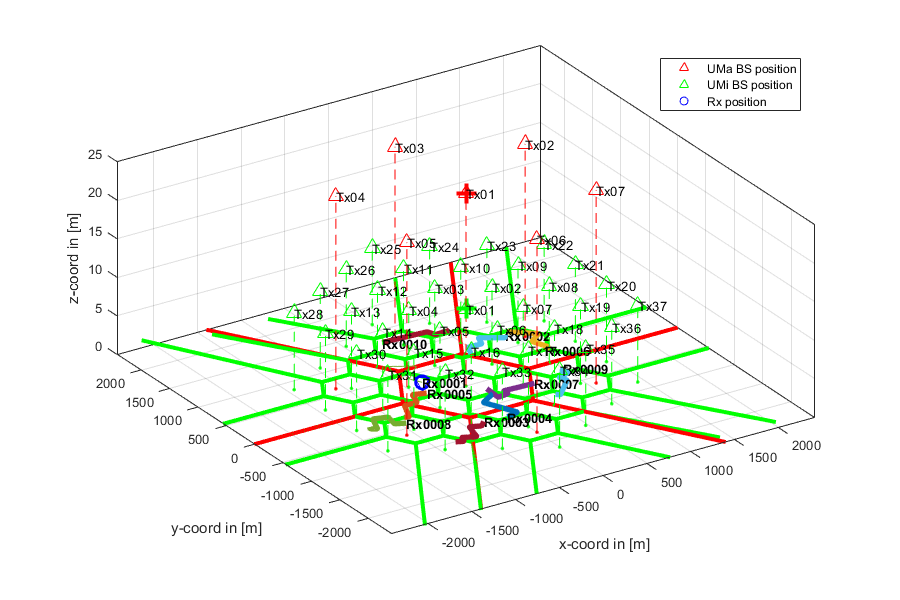
\includegraphics[width=\linewidth]{imagenes/muestra_visualizacion.png}
	\caption{Muestra de la visualización mejorada que implementa el simulador.}
	\label{fig:muestra_visualizacion}
\end{figure}

Gracias a todas estas implementaciones y funcionalidades, \textit{5Gneralife} es capaz de generar un entorno típico de 5G donde conviven celdas de distintos tipos, a altas frecuencias y altos anchos de banda, lo que permite evaluar el comportamiento de una red heterogénea realista con detalles lo suficientemente precisos como para que su comportamiento sea similar a una implementación del mismo tipo. 

\subsection{Lista de mejoras}

Para llegar al simulador se ha elaborado un conjunto de mejoras de \textit{QuaDRiGa} que, implementadas en su conjunto, resultan en \textit{5Gneralife}. Esto implica la elaboración de una nueva clase y de más de una decena de funciones que serán expuestas en la sub-sección de estructura y posteriormente, explicadas con detalle en la sección dedicada a la implementación.

A grandes rasgos, todas estas mejoras se pueden resumir en en el siguiente listado:

\begin{itemize}
    \item \textbf{Mejora 1:} Recopilación de variables de entrada intuitiva y de forma gráfica. Ampliación de parámetros de simulación como ruido o ancho de banda.
    \item \textbf{Mejora 2:} Combinación de celdas de modo que ahora los usuarios en ambas capas de simulación son los mismos. En este simulador, las capas no son independientes. Esto implica que se consigue una implementación de receptores con interfaz dual, una para cada banda de radio, y que no es necesario crear una capa de simulación para cada celda.
    \item \textbf{Mejora 3:} Inclusión de modelado de potencia de transmisión. Los coeficientes de canal que el generador calculaba se encontraban normalizados y no tenían en cuenta potencias de transmisión. Ahora, se ha añadido la implementación de dichas potencias para poder ajustarlo de acuerdo a los estándares que se deseen.
    \item \textbf{Mejora 4:} Criterios de emparejamiento. \textit{QuaDRiGa} no incluye ninguna herramienta que permita decidir criterios de emparejamiento, solamente calcula coeficientes de canal para todos los enlaces posibles -o bien, los enlaces que el usuario establezca manualmente-. El simulador, sin embargo, implementa algoritmos de decisión de enlaces de acuerdo a dos criterios actualmente: celda de la que se obtiene la mayor SINR y celda más cercana.
    \item \textbf{Mejora 5:} Post-procesado de los coeficientes de canal generados. Se han desarrollado funciones para el cálculo de potencia de recepción y de la SINR incluyendo el ruido térmico como componente, así como la capacidad de canal asignada a cada receptor.
    \item  \textbf{Mejora 6:} Visualización mejorada del escenario de simulación e inclusión de visualización de variables de salida. Se han añadido variables de salida como capacidad de canal asignada a cada receptor, SINR o potencia de recepción.
    \item \textbf{Mejora 7:} Interfaz gráfica de usuario para introducción de variables de entrada y para visualización de variables de salida.
    
\end{itemize}

\subsection{Modo de uso}

El uso del simulador es sencillo y no requiere de amplios conocimientos para llevar a cabo una simulación. Basta con ejecutar mediante Matlab el fichero \textit{main.m}, el cual se trata de un \textit{script} que se encarga de llamar, paso por paso, todas las funciones y recursos necesarios. El único requisito es que el fichero \textit{main.m} se encuentre en el directorio raíz del programa, junto a los dos directorios \textit{src} y \textit{quadriga\_src} como aparece en la Figura \ref{fig:directorio}:

\begin{figure}[h!]
	\centering
    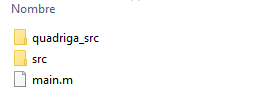
\includegraphics{imagenes/directorio.PNG}
	\caption{Directorio de instalación del simulador.}
	\label{fig:directorio}
\end{figure}

Tras ejecutarlo, se abrirá la primera de las dos interfaces gráficas de las que consta el programa. En ella, se debe introducir un total de x parámetros, entre ellos, el número de celdas de cada tipo con su respectiva frecuencia, número de usuarios, distancia recorrida por ellos, ancho de banda... Todos estos parámetros pueden verse en la Figura \ref{fig:interfaz_parametros} y se explicarán con detalle en las secciones dedicadas al diseño y a la implementación.

\begin{figure}[h!]
	\centering
    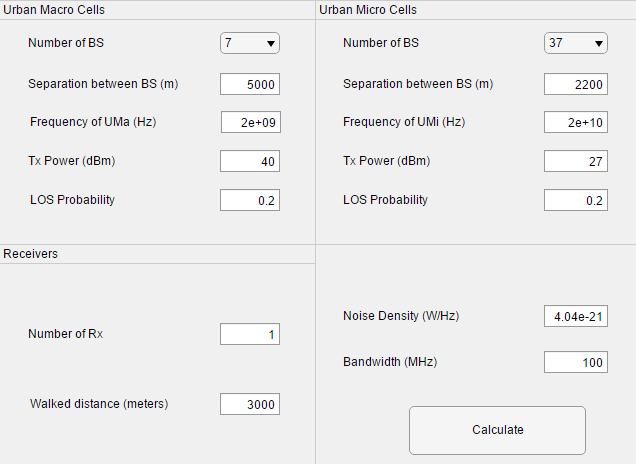
\includegraphics[width=\linewidth]{imagenes/interfaz_parametros.PNG}
	\caption{Interfaz de introducción de parámetros de simulación.}
	\label{fig:interfaz_parametros}
\end{figure}

La interfaz cuenta por defecto con unos parámetros que se han considerado estándar para una simulación 5G. El coste computacional y, por tanto, el tiempo de ejecución es directamente proporcional al número de estaciones base, de receptores y de la distancia recorrida por ellos. En el Capítulo \ref{cap.pruebas} se llevarán a cabo una serie de pruebas que mostrarán con detalle cómo varían los tiempos de ejecución en función de la exigencia del entorno simulado.

Una vez completa la simulación, se mostrará la segunda ventana gráfica donde se puede realizar las representaciones oportunas. En concreto, se pueden visualizar los valores de SINR, potencia de recepción, emparejamientos y capacidad de canal asignada a cada uno de los receptores durante su recorrido, para los casos de macro-celda y micro-celda, y para dos criterios de emparejamiento posibles: la celda de mayor SINR o la celda más cercana -Figura \ref{fig:interfaz_visualizacion}-. Además, es posible representar varios datos en la misma figura a través del \textit{checkbox} que incorpora.

\begin{figure}[h!]
	\centering
    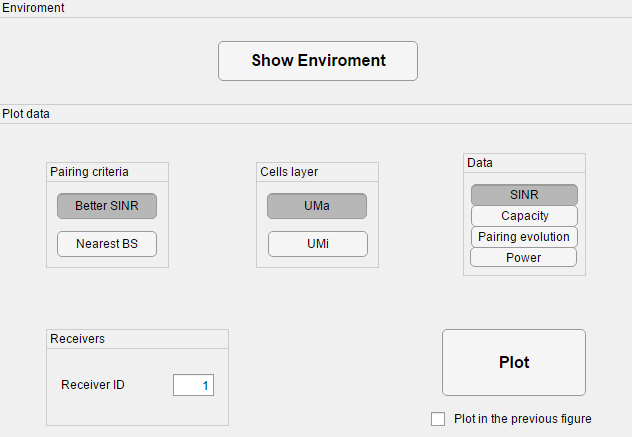
\includegraphics[width=\linewidth]{imagenes/interfaz_visualizacion.PNG}
	\caption{Interfaz de visualización de valores para las variables de salida.}
	\label{fig:interfaz_visualizacion}
\end{figure}

Una vez completa la simulación, si se atiende al \textit{workspace} de Matlab, se puede observar que se puede tener acceso a las variables de salida generadas -Figura \ref{fig:workspace}-. La naturaleza, estructura y contenido de las mismas se detallará en las secciones dedicadas a ello. Sin embargo, conviene tener en cuenta que se pueden almacenar en el disco duro a través del comando:

\begin{lstlisting}[style=Matlab-editor, basicstyle=\tiny]
save <nombre_de_fichero_de_salida>.mat
\end{lstlisting}

\begin{figure}[h!]
	\centering
    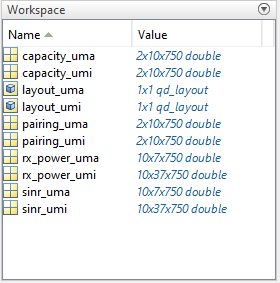
\includegraphics{imagenes/workspace.PNG}
	\caption{Workspace de Matlab tras la ejecución de una simulación.}
	\label{fig:workspace}
\end{figure}

Esto es especialmente útil cuando se quiere realizar una comparativa entre distintas simulaciones, ya que, en la actualidad, \textit{5Gneralife} solo admite la comparativa entre parámetros de salida de una misma simulación. Se estima que el fichero de salida adquiere un tamaño medio de 10 MB.

\section{Diseño}

\subsection{Planificación y concepción inicial}

Para justificar la implementación es necesario conocer previamente el planteamiento de su diseño y el proceso de concepción del mismo, puesto que una planificación debidamente estudiada es el método más eficiente para obtener un resultado de desarrollo satisfactorio.

Por ello, esta sección está dedicada a exponer las decisiones que se tomaron en la etapa de planteamiento y el motivo por el que se tomaron las mismas. De igual modo, también se justificarán los descartes de funcionalidades y simplificaciones que se adoptaron durante el proceso de implementación.

Si bien el proyecto contaba con unos objetivos flexibles desde el primer momento, como se comentaba en el Capítulo \ref{cap.requisitos}, existía una serie de requisitos para considerar el proyecto como satisfactorio una vez dada su finalización.

Estos requisitos surgen del estudio de los principales simuladores 5G existentes en la actualidad. De un rápido repaso al estado del arte del Capítulo \ref{cap.estado del arte} se puede concluir que éxito una basta gama de simuladores, pero cada uno se encuentra orientado a un propósito: desde simuladores técnicos especialmente diseñados para simulaciones que cumplan con ciertos estándares, hasta simuladores que tiene su propio modelado minimalista del comportamiento del canal y se centran en la evolución temporal de los receptores.

Sin embargo, en el momento de evaluación de alternativas no existía un simulador que reúna las principales características de todos ellos, un simulador completo que integre las normativas de simulaciones junto a evolución temporal, correlación entre cálculos y especificaciones propias de 5G como alta frecuencia o sistemas MIMO.

Es como surge \textit{5Gneralife}, el cual se concibió como una alternativa a los ya existentes, al pretender incluir evolución temporal junto a modelados de acuerdo a las diferentes normativas de simulación y la posibilidad de convivencia de celdas de distinta naturaleza en un entorno de \acs{hetnet}s.

La idea básica era basarse en la potencia que ofrece \textit{QUaDRiGa} para implementar las funciones necesarias, de modo que \textit{5Gneralife} fuera capaz de realizar un seguimiento de la señal recibida por todos los usuarios en cada instante de tiempo para todas las celdas, las cuales pueden ser de cualquier naturaleza a priori. Además, es crucial para simulaciones en 5G la incorporación de posibilidad de calcular resultados a muy altas frecuencias, puesto que la mayor novedad que incluye 5G es la de trabajar a frecuencias del orden de diez veces mayores que las que se han estado trabajando hasta ahora, así, se consiguen unas mayores tasas de transferencia y capacidades, aspecto del que se carecen estudios de comportamiento hasta la fecha.

Así, este simulador podría contribuir a realizar una mejor toma de contacto con este nuevo paradigma, junto a técnicas avanzadas como MIMO, ICIC, emparejamientos sofisticados de terminal-estación base u optimización de la planificación.

Sin embargo, por motivos de complejidad y por haberse considerado fuera del alcance de un Trabajo de Fin de Grado individual, se han descartado estas funcionalidades avanzadas y se han sustituido por simplificaciones como enlaces SISO, interfaz de conexión dual sin decisión de banda a la que conectar, emparejamientos basados en parámetros básicos y planificación geométrica con reutilización de frecuencias unitario.

Su diseño inicial se pensó como un solo \textit{script} para Matlab que integrara en él todos los cálculos y llamadas al generador de canal, cuyos resultados se pudieran estudiar a través de la línea de comandos. No obstante, al ver la relevancia de las implementaciones y de su posible mejora y escalabilidad, se decidió re-estructurar el trabajo para que fuera modular, con un arquetipo que utiliza funciones para labores específicas, y que implementa una nueva clase para reunir en un solo objeto todos los parámetros, dando así lugar a la estructura final que se presenta a continuación.

\subsection{Estructura final}

El simulador consta de un total de 14 ficheros desarrollados exclusivamente para su implementación, más todos los ficheros por los que \textit{QuaDRiGa} está constituido. 
De estos 14 ficheros, uno de ellos es el archivo principal, \textit{main.m}, que es el que se debe ejecutar para iniciar el simulador. Por otro lado, dos de los otros ficheros corresponden a las dos ventanas por las que está formada la interfaz gráfica. El resto son funciones dedicadas a realizar cálculos específicos, desde el cálculo de la SINR hasta la generación de coeficientes de canal, o bien, dedicadas a representar gráficamente los resultados.

De este modo, se puede realizar un diagrama de flujo en el que se detallan los pasos que realiza el simulador a la hora de ejecutarse, mostrando el orden de las funciones de las que se sirve en cada paso, como se especifica en la Figura \ref{fig:diagrama_simulador}:

\begin{figure}[h!]
	\centering
    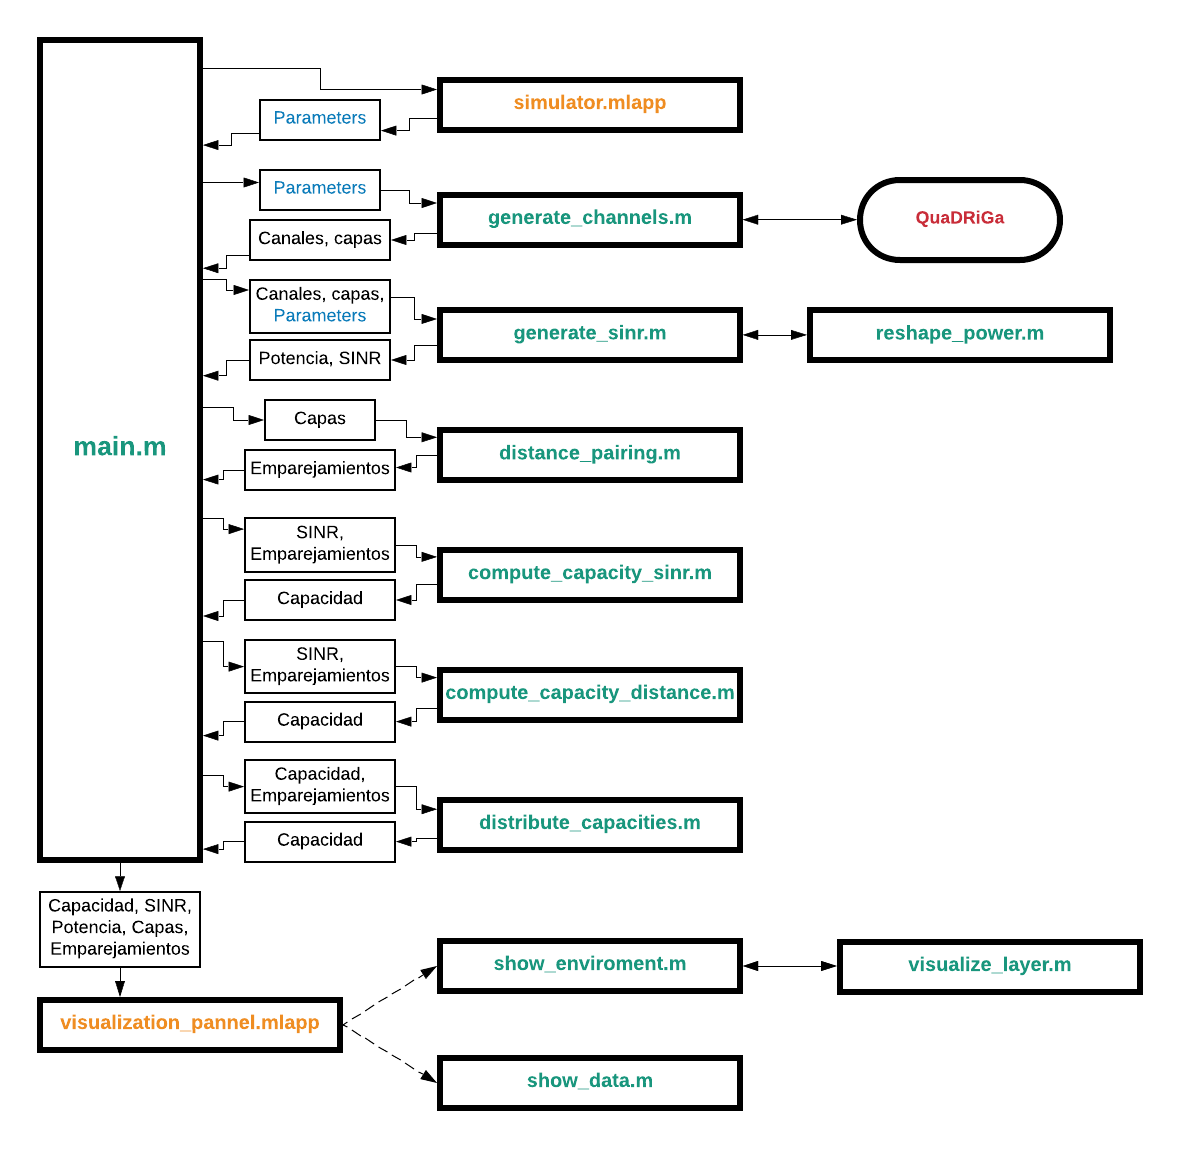
\includegraphics[width=\linewidth]{imagenes/diagrama_simulador.png}
	\caption{Diagrama de flujo del simulador.}
	\label{fig:diagrama_simulador}
\end{figure}

Además, se puede completar el anterior diagrama mostrando las etapas en las que se hace uso del cómputo de \textit{QuaDRiGa}, añadiendo las clases de las que se hace uso en cada momento -Figura \ref{fig:diagrama_simulador_completo}-:

\begin{figure}[h!]
	\centering
    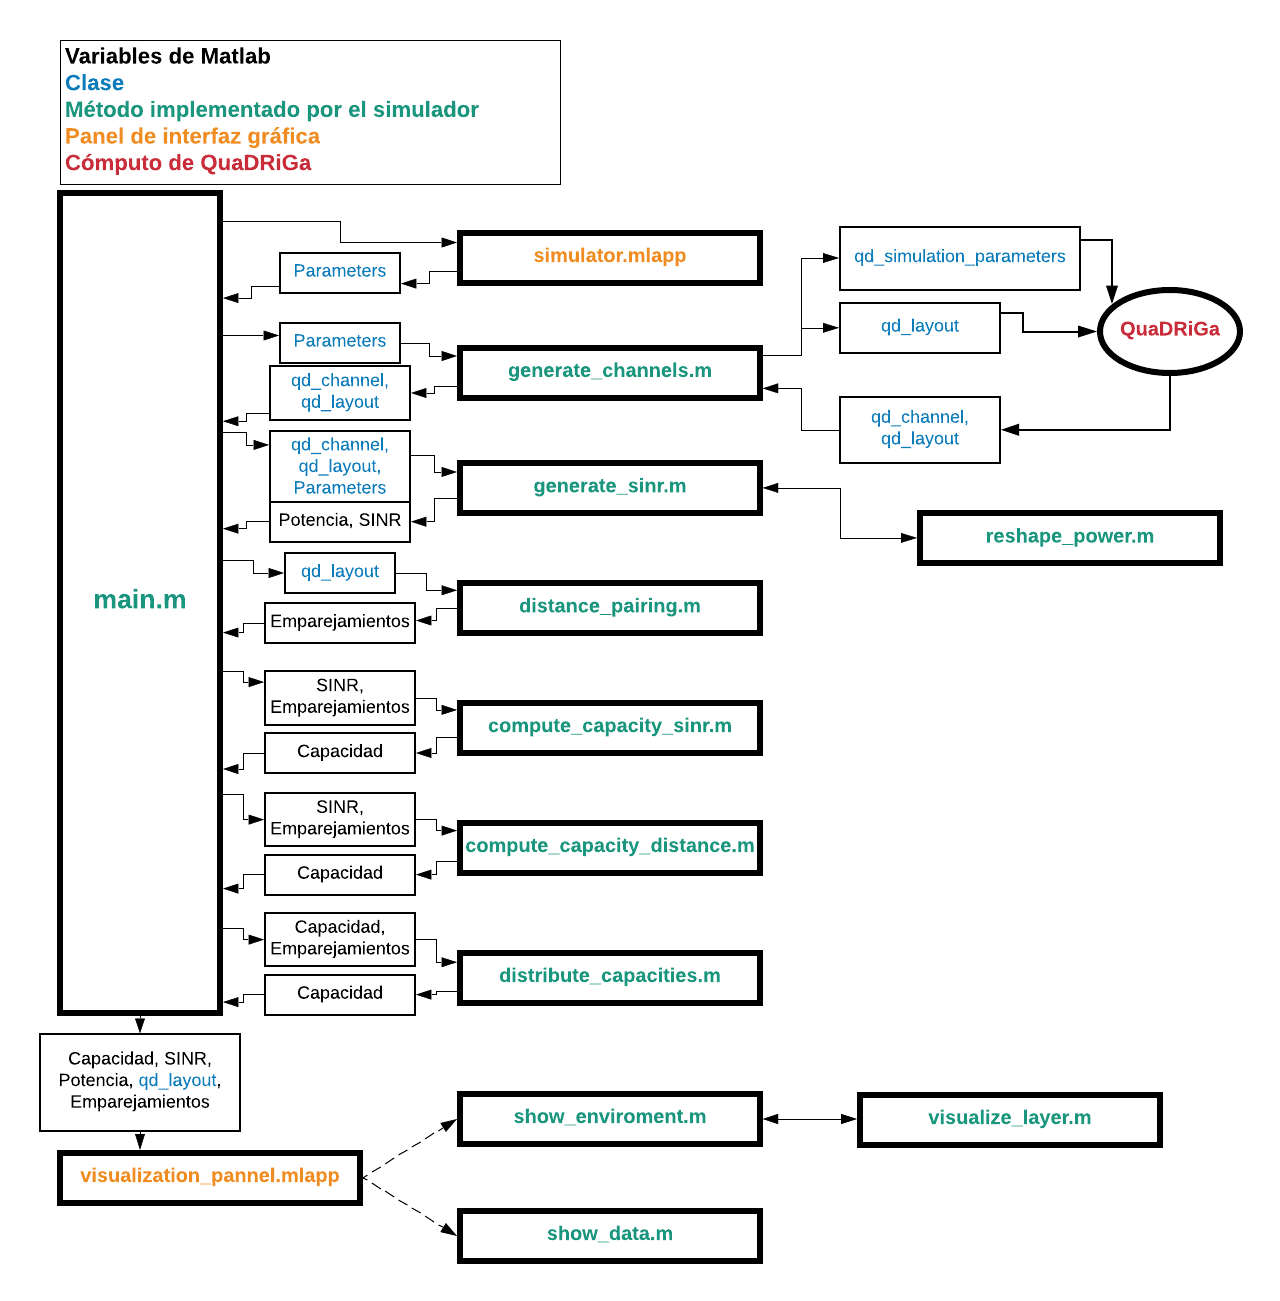
\includegraphics[width=\linewidth]{imagenes/diagrama_simulador_completo.png}
	\caption{Diagrama de flujo del simulador incluyendo las clases de \textit{QuaDRiGa}.}
	\label{fig:diagrama_simulador_completo}
\end{figure}

Como se puede observar, cada uno de los módulos en verde o en naranja, es decir, los implementados por el usuario, están dedicados a una tarea específica y son totalmente sustituibles y escalables. De este modo se facilitan las futuras implementaciones, como podría ser un tercer criterio de emparejamiento, una forma distinta de calcular la SINR o simplemente un nuevo parámetro como atributo de la clase \textit{Parameters}.

Por lo general, cada uno de los anteriormente citados módulos implementa una o varias mejoras de las listadas en la anterior sub-sección, o forman parte de una de ellas. El modo de implementación de dichas mejoras así como el código de las mismas se detallará en la siguiente sección. 

\section{Implementación}

\subsection{Implementación del diseño}

Antes de realizar el desarrollo de las funciones propias del simulador, es necesario llevar a cabo un desarrollo del diseño propuesto a partir de los elementos disponibles por parte de \textit{QuaDRiGa}. Esto implica modificar, generar y establecer una serie de parámetros que no son visibles para el usuario, puesto que en la fase de diseño se decidió que no sean modificables, con la finalidad de establecer las bases de la simulación y de este modo ajustar todas las configuraciones para que sean compatibles con 5G y el simulador posteriormente desarrollado.

En primer lugar, se ha establecido como único modelo de canal el de 3GPP TR-38.901 \cite{3gpphighfreq} el cual establece un modelado para el canal de radio de la comunicación para altas frecuencias. Aunque \textit{QuaDRiGa} ya de por sí incorpora soporte para la incorporación de este modelo de canal sin nada más que especificar que se desea utilizar el mismo, conviene conocer los detalles de lo que implica utilizar este modelado.

\begin{table}[h!]
\centering
\caption{Implicaciones de adoptar el estándar de 3GPP TR 38.901 para las implementaciones}
\label{tab:tr38901}
\begin{tabular}{|l|m{4cm}|m{4cm}|} \hline
\textbf{Característica} & \textbf{Micro-celda urbana}                                                              & \textbf{Macro-celda urbana}                                                              \\ \hline
Capa de celdas          & Hexagonal con 3 sectores por cada estación base. Distancia mínima entre celdas de 200 m. & Hexagonal con 3 sectores por cada estación base. Distancia mínima entre celdas de 500 m. \\ \hline
Visión directa          & LOS y NLOS.                                                                              & LOS y NLOS.                                                                              \\ \hline
Altura de BS            & 10 m.                                                                                    & 25 m.                                                                                    \\ \hline
Antenas                 & 3 sectores por base.                                                                     & 3 sectores por base.                                                             \\ \hline       
\end{tabular}
\end{table}

Según la Tabla \ref{tab:tr38901} de implicaciones, se establece una altura de 10 m y de 25 m para las estaciones base de micro-celdas y macro-celdas respectivamente, a la misma vez que el modelado de las antenas se hacen en tres sectores 

Por otro lado, en cuanto a la antena de transmisión, se ha utilizado la misma para ambos tipos de estación base. Se trata de una antena sectorial de aproximadamente 120º de apertura, replicada dos veces más para conseguir una cobertura total de 360º. Esta antena es compatible con todos los rangos de frecuencia por lo que es reutilizable para cualquier tipo de estación base. Se puede observar un plano de su radiación normalizada en dos dimensiones en la Figura \ref{fig:radiacion}, teniendo en cuenta que esta variará según la frecuencia y la potencia de transmisión.

\begin{figure}[h!]
	\centering
    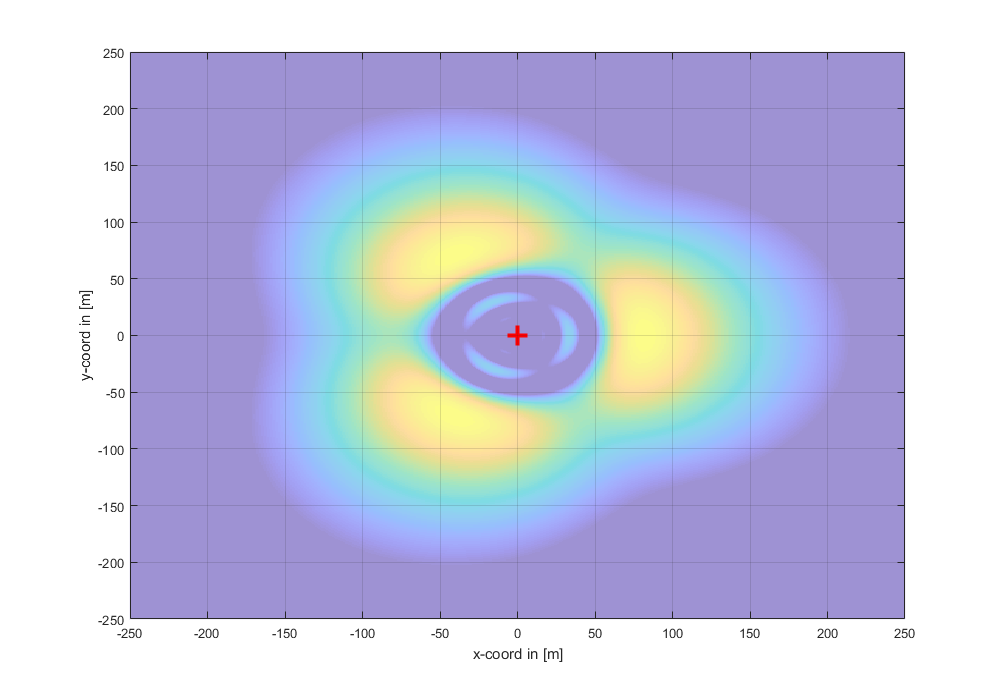
\includegraphics[width=\linewidth]{imagenes/articulo_radiacion.png}
	\caption{Esquema de radiación de la antena utilizada para los transmisores.}
	\label{fig:radiacion}
\end{figure}

Estas configuraciones para hacer posible su compatibilidad se han implementado a través del siguiente código en sus pertinentes ficheros:

\begin{lstlisting}[style=Matlab-editor, basicstyle=\tiny]
scenarios_uma = {'3GPP_38.901_UMa_LOS', '3GPP_38.901_UMa_NLOS'};
scenarios_umi = {'3GPP_38.901_UMi_LOS', '3GPP_38.901_UMi_NLOS'};

%% Antennas
aMT = qd_arrayant('omni');
aBS = qd_arrayant ('multi', 8, 0.5 , 12 );
aBS.combine_pattern;
aBS_umi = aBS.copy;

layout_uma = qd_layout.generate ('regular', params.number_of_uma, params.dist_between_uma, aBS);
layout_umi = qd_layout.generate ('regular', params.number_of_umi, params.dist_between_umi, aBS_umi);

layout_uma.tx_position(3,:) = 25; % 25 m BS height
layout_uma.set_scenario('3GPP_38.901_UMa',[],[],0,1-los_uma);

layout_umi.tx_position(3,:) = 10; % 10 m BS height
layout_umi.set_scenario('3GPP_38.901_UMi',[],[],0,1-los_umi);
\end{lstlisting}

\subsection{Implementación de mejoras}

A grandes rasgos, se puede considerar el simulador como una caja negra en la que se introducen una serie de parámetros sobre la simulación deseada y esta devuelve los valores numéricos sobre diversas características del entorno simulado. Debido a la gran cantidad de parámetros de entrada y de salida disponibles, la mejor forma de tenerlos en consideración es a través de un esquema gráfico:

\begin{figure}[h!]
	\centering
    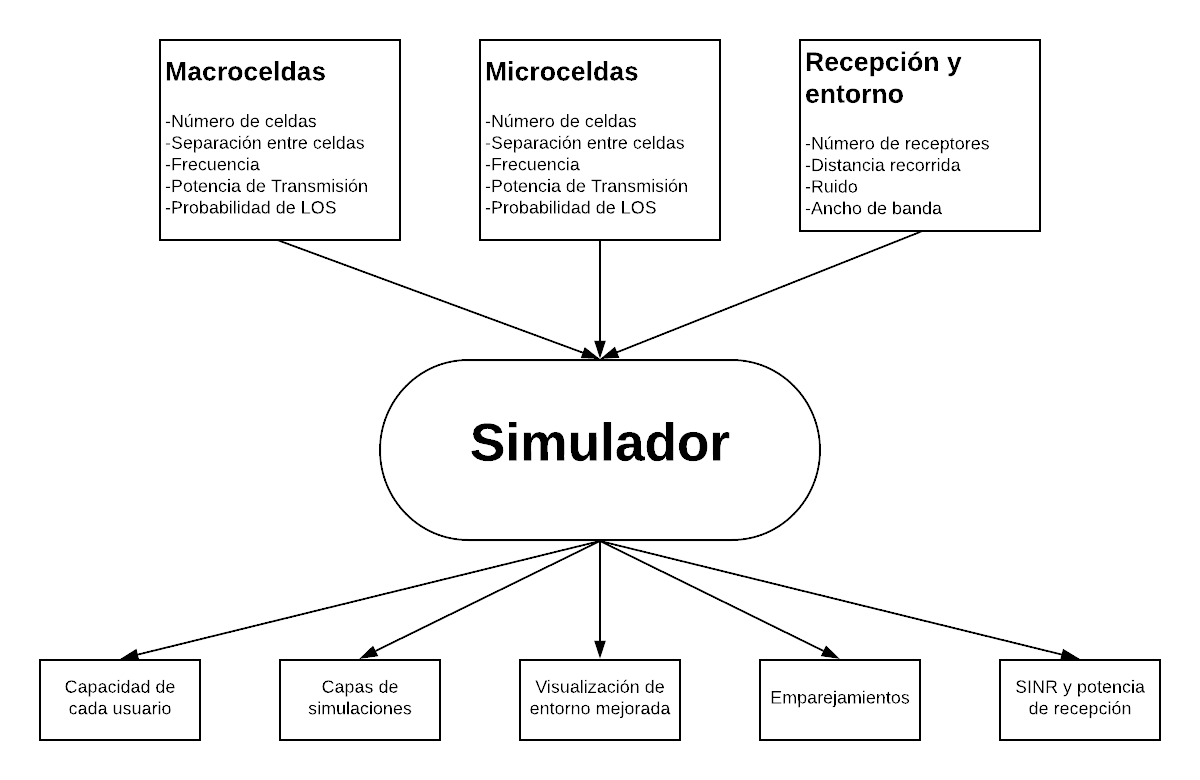
\includegraphics[width=\linewidth]{imagenes/cajanegra_simulador.png}
	\caption{Esquema de la relación de entrada y salida del simulador.}
	\label{fig:cajanegra}
\end{figure}

Estos resultados se obtienen gracias al desarrollo de las mejoras con respecto a \textit{QuaDRiGa}. Gracias a ello, el software resultante puede considerarse un simulador completo y funcional con características propias de nivel de enlace y de nivel de sistema, puesto que es capaz de evaluar emparejamientos y establecimientos de enlace a la misma vez que calcula parámetros de utilización como la capacidad o \textit{throughput}.

Centrándonos en la implementación, esta se puede resumir detallando las siete mejoras desarrolladas que se han enunciado con anterioridad, puesto que son las tareas donde se ha centrado la labor de programación, haciendo especial hincapié en ampliar las características de \textit{QuaDRiGa}. Por ello, a continuación se detalla el procedimiento de implementación de cada una de las mejoras con la finalidad de ilustrar la tarea de desarrollo y sus resultados. 

En cuanto al código, resulta importante mencionar que ha sido completamente escrito en inglés para facilitar su distribución y uso, puesto que existe una gran comunidad científica internacional que ha utilizado \textit{QuaDRiGa} para sus investigaciones y es probable que \textit{5Gneralife} les resulte atractivo. Además, así se posibilita una mayor participación en la plataforma colaborativa donde ha sido publicado el código. El mismo ha sido completamente documentado y comentado, y utiliza técnicas de programación como nombres de variables y de funciones descriptivos para facilitar su comprensión mientras se revisa y/o modifica.

\paragraph{Implementación de la Mejora 1: Recolección de datos de entrada} \mbox{} \\

Una de las problemáticas que se encontraron acerca del uso de \textit{QuaDRiGa} fue precisamente el establecimiento de parámetros de simulación. Este generador incorpora los parámetros en distintas clases de modo que es necesario especificarlos uno por uno a la misma vez que se atiende a qué clase corresponde cada parámetro.

Por ello, se ha decidido solventar este problema unificando todos los parámetros que se han considerado interesantes para su variación en una nueva clase implementada, mientras que aquellos parámetros que se ha decidido que permanezcan constantes, se han excluido de dicha clase y se han establecido a lo largo del código de todo el simulador de forma estática.

Esta implementación se ha llevado a cabo mediante la clase \textit{Parameters}, contenida en el fichero \textit{Parameters.m}. En esta versión inicial del simulador, implementa un total de 14 atributos, uno por cada parámetro de entrada, dos métodos que tienen como finalidad la de convertir la potencia de transmisión a unidades lineales y por último un constructor.

Se ha optado por establecer como públicos todos los atributos y métodos por simplificación, en lugar de implementar por cada uno de los atributos un método \textit{get} y otro método \textit{set}, que son típicos cuando se utiliza el paradigma de programación orientada a objetos. De este modo, se puede acceder y modificar directamente estos parámetros. Se puede observar la implementación de sus atributos y métodos en el siguiente código:

\begin{lstlisting}[style=Matlab-editor, basicstyle=\tiny]
    properties
        freq_uma; % UMa Frequency in Hz
        freq_umi; % UMi Frequency in Hz
        number_of_uma; % Number of Macro-cells
        number_of_umi; % Number of Micro-cells
        dist_between_uma; % Distance between UMa cells center
        dist_between_umi; % Distance between UMi cells center
        number_of_rx; % Number of Mobile Terminals
        walked_distance; % Distance that Mobile Terminals will walk in meters
        tx_power_uma; % Transmit Power of UMa BS in dBm
        tx_power_umi; % Transmit Power of UMi BS in dBm 
        BW; % Asigned bandwidth to each BS in MHz
        No; % Noise in W/Hz
        los_uma; % LOS probability for UMa enviroment
        los_umi; % LOS probability for UMi enviroment
    end
    
    methods
        function pow = get_lin_pow_uma(obj)
            pow = 10^(obj.tx_power_uma/10); % Power in W
        end
        function pow = get_lin_pow_umi(obj)
            pow = 10^(obj.tx_power_umi/10); % Power in W
        end
    end
\end{lstlisting}

\paragraph{Implementación de la Mejora 2: Combinación de capas de simulación independientes} \mbox{} \\

El mayor impedimento con el que cuenta \textit{QuaDRiGa} a la hora de simular entornos heterogéneos es la independencia entre sus capas de simulación y la imposibilidad de combinarlas. Recuérdese que el entorno de simulación se encuentra implícito en el objeto de los receptores y no en los de las estaciones base, puesto que no existe un objeto dedicado a ellas. De nada sirve simular una capa de macro-celdas con usuarios aleatorios si se necesita simular una segunda capa de micro-celdas que cuenta con otros usuarios distintos aleatorios.

Por ello, se ha utilizado una versión modificada del ejemplo que se mostraba en el Capítulo \ref{cap.quadriga} para generar las dos capas de simulación y sus respectivos coeficientes de canal. Esta función funciona del mismo modo que el ejemplo anterior, con la salvedad de que se repite una segunda vez para la capa de micro-celdas. Una vez que ambas capas son creadas, se procede a crear uno a uno el objeto \textit{qd\_track} que modela el movimiento de los receptores por las calles de Berlín a lo largo de la distancia especificada por el usuario del simulador. Lo que hace especial esta parte es que este objeto, antes de serle asignado un entorno de simulación, es copiado a ambas capas de simulación. De este modo, ambas capas tendrán un usuario idéntico, con el mismo recorrido, pero con distintos segmentos, distintos puntos de transición de LOS a NLOS y viceversa, y distintos tipos de celda asignados:

\begin{lstlisting}[style=Matlab-editor, basicstyle=\tiny]
prob_uma = [los_uma, 1-los_uma];
prob_umi = [los_umi, 1-los_umi];

scenarios_uma = {'3GPP_38.901_UMa_LOS', '3GPP_38.901_UMa_NLOS'};
scenarios_umi = {'3GPP_38.901_UMi_LOS', '3GPP_38.901_UMi_NLOS'};

%% Write all streets in one layout

for a = 1 : params.number_of_rx
    trk = qd_track('street', params.walked_distance, randi(360), 50, 87, 83, 10, 0.85); % Street
    trk.initial_position = layout_uma.rx_position(:,a); % Strat-pos
    trk.name = layout_uma.rx_name{a};  % Unique name
    layout_uma.track(1,a) = trk{1}.copy; % Assign to layout
    layout_uma.track(1,a).set_scenario( scenarios_uma, prob_uma, 10 ,30, 12 );
    layout_umi.track(1,a) = trk{1}.copy;
    layout_umi.track(1,a).set_scenario( scenarios_umi, prob_umi, 10 ,30, 12 ); % Segments
end
\end{lstlisting}

\paragraph{Implementación de la Mejora 3: Modelado de potencia de transmisión y de SINR} \mbox{} \\

La única salida que ofrece \textit{QuaDRiGa} es la de un objeto que entre su contenido se encuentran los coeficientes de canal del enlace -clase \textit{qd\_channel}-.  Estos coeficientes pretenden modelar las comunicaciones del canal de modo que cada comunicación individual entre un transmisor y un receptor tenga un coeficiente característico que contenga la relación entre la señal emitida y la recibida.

En la Figura \ref{fig:esquema_comunicacion} se puede apreciar el esquema de una situación típica en la que un transmisor, $Tx_1$, se comunica con \textit{M} receptores. En total habrá una cantidad de \textit{M} enlaces establecidos, uno por cada receptor, en los que la amplitud de la señal se verá afectada así como su fase una vez recibida.

\begin{figure}[h!]
	\centering
    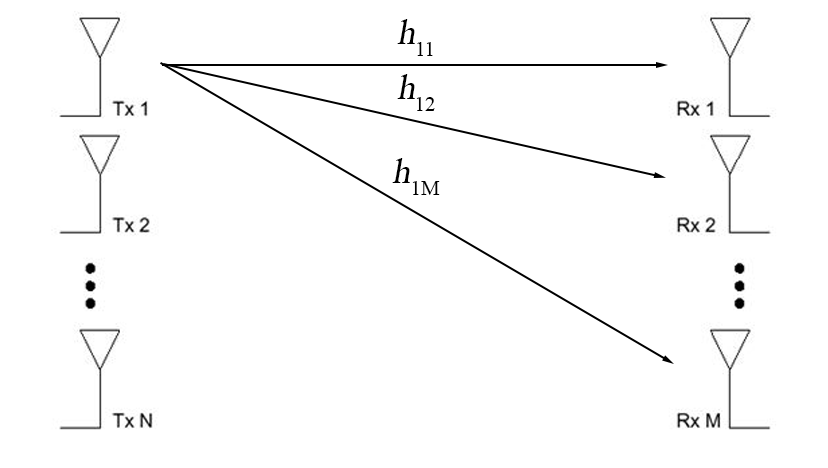
\includegraphics[width=0.85\linewidth]{imagenes/esquema_comunicacion.png}
	\caption{Esquema de comunicación en un entorno con varios receptores y emisores.}
	\label{fig:esquema_comunicacion}
\end{figure}

Por tanto, se puede considerar el canal como una función de transferencia $H$ que modifica la amplitud y la fase de la señal \cite{modelado}. Es decir, se trata de una función de transferencia compuesta por una matriz de dimensiones \textit{NxM}, siendo \textit{N} el número de transmisores y \textit{M} el número de receptores, cuyos coeficientes son números complejos con un módulo que resulta en la relación entre amplitudes, y con una fase que incorpora el desfase entre señales -Figura \ref{fig:matrizcanal}-.

\begin{figure}[h!]
	\centering
    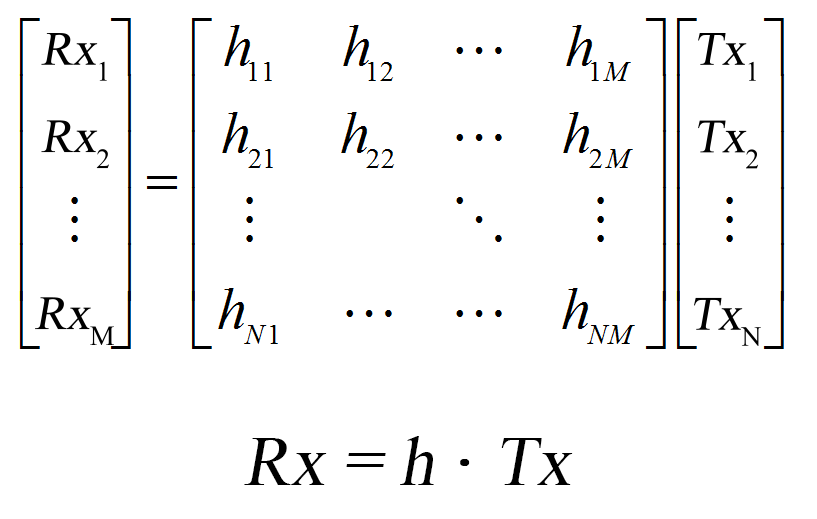
\includegraphics[width=0.75\linewidth]{imagenes/matriz_canal.png}
	\caption{Matriz del canal y relación entre coeficientes.}
	\label{fig:matrizcanal}
\end{figure}


Donde $h_ij$ es un coeficiente complejo que contiene la información de la relación entre la señal transmitida por el transmisor $Tx_i$ y la señal recibida por el receptor $Rx_j$ \cite{matrizcanal}. \textit{QuaDRiGa} almacena estos coeficientes en la matriz de cuatro dimensiones que se describía en el Capítulo \ref{cap.quadriga}. Dicha matriz se almacena en el atributo \textit{coeff} de la clase \textit{qd\_channel}.

Aunque el desfase puede resultar en interferencias destructivas debido al modelo de rayo de 20 trayectorias, cuya superposición pueda resultar en una interferencia consigo misma, para la estimación de la potencia se ha despreciado este posible efecto y solamente se ha atendido al módulo de los coeficientes.

Ya que \textit{QuaDRiGa} no implementa la posibilidad de inclusión de potencia de transmisión, se ha realizado una implementación sencilla de cálculo de potencia de recepción a través del módulo de la matriz de canal. En concreto, teniendo en cuenta que se trabaja con unidades lineales, la potencia de recepción se encuentra definida por:

$$ P_{Rx_i} = |h_{ij}|^2 * P_{Tx_j} (W) $$

Para \textit{5Gneralife} se ha implementado esta funcionalidad a partir de la introducción de la potencia de transmisión en dBm y convirtiendo dicho valor a unidades lineales -vatios- a través del método dedicado a ello de la clase \textit{Parameters}. El cálculo de potencias se realiza para cada uno de los enlaces, esto quiere decir que se necesita un total de interacciones igual al producto del número de receptores, el número de transmisores total y el número de muestras tomadas -por defecto, una muestra por cada metros recorrido-. Estos cálculos han sido implementados en la función \textit{generate\_sinr} que está dedicada precisamente al cálculo de potencia de recepción y a la SINR a través de la debida extracción de los coeficientes de canal:

\begin{lstlisting}[style=Matlab-editor, basicstyle=\tiny]
for a = 1 : number_of_rx
    power = zeros( layout.no_tx*3 , no_snap_per_track );
    for builder = 1 : layout.no_tx
        power_calc = abs(channel(a,builder).coeff).^2;
        power_calc = sum( power_calc, no_sectors_per_bs );
        power_calc = reshape( power_calc, no_sectors_per_bs, no_snap_per_track );         % 3 sectors per BS

        index = (builder-1)*no_sectors_per_bs+1 : builder*no_sectors_per_bs;
        power(index,:) = power_calc * tx_power;
    end

    rx_aux(a, :, :) = power;
end
\end{lstlisting}

Esto realiza un cálculo de la potencia para cada receptor en cada instante de tiempo. Sin embargo, la característica más interesante a la hora del estudio de una red de comunicaciones inalámbricas no es la potencia de recepción, sino la relación de esta frente al ruido y al resto de señales del entorno, también conocida como SINR. Por ello, gracias a la integración de ruido térmico como parámetro de entrada, se puede modelar este parámetro a partir de la recopilación de todas las potencias de transmisión \cite{capacity}:

\[SINR_i = \frac{P_{BS_i}}{N_{o} - P_{BS}(i) + \sum_{j = 1}^{N} P_{BS_j}}\]

Siendo $P_{BS_i}$ la potencia recibida por la estación base \textit{i}, $N_o$ el ruido térmico en W y $N$ el número de estaciones base a la misma frecuencia que la estación base \textit{i}.

Esta implementación se ha realizado mediante el cálculo iterativo de la SINR para todos los receptores considerando todos los posibles casos de enlace, con la finalidad de determinar en cada instante de tiempo la SINR de todas las estaciones base y así poder compararlas entre sí, lo cual facilita la tarea de elección de la mejor SINR para emparejamientos:

\begin{lstlisting}[style=Matlab-editor, basicstyle=\tiny]
for i = 1:number_of_rx
    aux = rx_aux(i,:,:);
    aux = reshape(aux, [layout.no_tx*3, no_snap_per_track]);
    current_rx_pow = reshape_power(aux);

    for j = 1:layout.no_tx
        for k = 1:no_snap_per_track
            sinr(i,j,k) = current_rx_pow(j,k) / ...
                (sum(current_rx_pow(:, k)) + No - current_rx_pow(j,k));
        end
    end

    sinr(i,:,:) = 10*log10(sinr(i,:,:));
    rx_power(i, :, :) = current_rx_pow;
end
\end{lstlisting}

\paragraph{Implementación de la Mejora 4: Criterios de emparejamiento} \mbox{} \\

Existe en la actualidad una gran diversidad de métodos de emparejamiento de terminales móviles que determinan la mejor estación base dependiendo de múltiples criterios. Este factor puede resultar decisivo en la eficiencia de la red y en posibles congestiones, puesto que determina con qué intensidad se está utilizando la infraestructura, sin dejar de tener en cuenta que los recursos de la red siempre son limitados.

Aunque la variedad de algoritmos de emparejamiento puede dar pie a un estudio mucho más exhaustivo, lo suficiente como para surgir otro proyecto independiente, para la implementación del simulador se ha decidido que, por limitación de tiempo y para priorizar otros aspectos del desarrollo, solamente se han tenido en cuenta dos criterios como se venía comentando anteriormente: emparejamiento con la estación base más cercana y emparejamiento con la estación base de mayor SINR recibida.

Para su implementación, simplemente se explora la matriz de SINR o la matriz de distancias, dependiendo del caso, con la finalidad de almacenar en una matriz de emparejamientos el índice de la estación base correspondiente. Esta selección se realiza a través de la función \textit{distance\_pairing} para el emparejamiento por distancia y mediante un sencillo recorrido del máximo de la variable SINR en el fichero principal de ejecución.

Emparejamiento por SINR:

\begin{lstlisting}[style=Matlab-editor, basicstyle=\tiny]
for j = 1:no_snap
    for i = 1:params.number_of_rx
        [~, pairing_uma(1,i,j)] = max( sinr_uma(i,:,j) );
        [~, pairing_umi(1,i,j)] = max( sinr_umi(i,:,j) );
    end
end
\end{lstlisting}

Emparejamiento por distancia:

\begin{lstlisting}[style=Matlab-editor, basicstyle=\tiny]
for i = 1:snap
    for j = 1:no_rx
        for k = 1:no_tx
            pos_rx = layout.track(j).positions(:,i) + layout.track(j).initial_position(:);
            pos_tx = layout.tx_position(:,k);
            distances(j,i,k) = sqrt(sum((pos_rx-pos_tx).^2));
        end
    end
end
    
for i = 1:snap
    for j = 1:no_rx
        [~, indice] = min(distances(j,i,:));
        pairing(j,i) = indice;
    end
end
\end{lstlisting}

\paragraph{Implementación de la Mejora 5: Cálculo capacidad de canal} \mbox{} \\

Uno de los factores en los que más énfasis se hace para futuras implementaciones de 5G es el de asignación de ancho de banda. Debido a las grandes tasas de transferencia que se espera y a la gran cantidad de usuarios, es primordial un reparto del ancho de banda disponible eficiente.

Para \textit{5Gneralife} se ha diseñado una mecánica de reparto de ancho de banda que se rige por la compartición equitativa por parte de todos los usuarios conectados a una misma celda o estación base, a la cual se ha pre-asignado un ancho de banda predeterminado de acuerdo con el parámetro especificado por el usuario del simulador.

Este ancho de banda asignado se encuentra directamente relacionado con una característica que afecta directamente a la experiencia del usuario: la tasa de transferencia máxima, también conocida como capacidad de canal o \textit{troughput}. Esta tasa de transferencia es un factor clave en usos de la red orientadas a multimedia, como vídeo o descargas, puesto que determinará el tiempo que tardará un fichero en descargarse o la calidad máxima que un \textit{streaming} de vídeo podrá adoptar para una calidad de servicio satisfactoria.

Para este simulador, se ha implementado la siguiente ecuación que se sirve de la SINR y del ancho de banda asignado a cierto usuario para determinar su máxima tasa de transferencia \cite{capacity}:

$$C = BW · \log_{2}( 1 + SINR(dB) ) (MBit/s) $$

Puesto que la SINR obtenida dependerá de la estación base o celda a la que se ha vinculado el receptor en cuestión, el cálculo dependerá estrechamente del criterio de emparejamiento. Por tanto, para un mismo receptor y una misma capa de simulación en un mismo instante de tiempo, se obtendrán dos valores de \textit{throughput} diferentes: uno para el caso de emparejamiento con la celda más cercana y otro para el caso de emparejamiento con la celda de mayor SINR.

Aunque resulta intuitivo que, puesto que la SINR está directamente relacionada con el resultado calculado de capacidad, la mayor capacidad se dará en el caso de conexión a la estación base de mejor SINR, existen casos en los que esta suposición no es correcta, puesto que el ancho de banda varía en función del número de terminales móviles conectados a la estación base estudiada. Por tanto, los resultados variarán sustancialmente dependiendo de si en el caso simulado existe congestión en una o más celdas.

La implementación de esta característica se ha llevado a cabo mediante las funciones \textit{compute\_capacity\_sinr} y \textit{compute\_capacity\_sinr}, dedicadas a calcular la capacidad en el caso de emparejamiento de la mejor SINR o de la menor distancia, respectivamente. Para ello, toman como parámetros de entrada la SINR anteriormente calculada, o bien, los objetos de capas para calcular la distancia hasta el centro de las celdas, dependiendo del caso, así como la matriz de emparejamientos.

Código de implementación para el caso de mejor SINR -\textit{compute\_capacity\_sinr}-:
\begin{lstlisting}[style=Matlab-editor, basicstyle=\tiny]
for i = 1:dimension(1)
    for j = 1:dimension(3)
        sinr_dist(i,j) = sinr(i, pairing(1, i, j), j);
    end
end
sinr_dist(sinr_dist < 0) = 0;
capacity(:,:) = BW*log2(1+sinr_dist);
\end{lstlisting}

Código de implementación para el caso de celda más cercana -\textit{compute\_capacity\_distance}-:
\begin{lstlisting}[style=Matlab-editor, basicstyle=\tiny]
for i = 1:dimension(1)
    for j = 1:dimension(3)
        sinr_dist(i,j) = sinr(i, pairing(2, i, j), j);
    end
end
sinr_dist(sinr_dist < 0) = 0;
capacity(:,:) = BW*log2(1+sinr_dist);
\end{lstlisting}

\paragraph{Implementación de la Mejora 6: Visualización mejorada} \mbox{} \\

Aunque esta no es una funcionalidad fundamental de los simuladores de comunicaciones, ya que estos suelen estar orientados a los estudios cuantitativos y la extracción de datos de los entornos generados, en numerosos casos resultan útiles las representaciones gráficas de las simulaciones en cuanto a disposición de elementos se refiere.

Sin embargo, al tratarse de un generador y modelador de canal generalista, las funciones que \textit{QuaDRiGa} relacionadas con la representación visual pueden resultar un poco escuetas e incompletas, sobre todo en casos con escenarios sobrecargados de usuarios, donde puede ser difícil visualizar dónde se encuentra el receptor en cuestión.

Por ello, aunque no sea una característica propia de un simulador técnico, se ha decidido emplear una porción del tiempo disponible para el proyecto en mejorar la visualización nativa de \textit{QuaDRiGa} e incorporar funciones como la de representar varias capas al mismo tiempo -antes solo se podían representar las capas individualmente ya que el método de representación estaba implementado en la clase \textit{qd\_layout}-, distinguir fronteras entre celdas -implementado gracias a la función de Matlab \textit{voronoi}- o representar la trayectoria de los receptores de una forma más estética, asignando también un color diferente a cada uno de ellos.

Esta mejora se ha implementado mediante una función dedicada exclusivamente a representar las dos capas de simulación en una misma figura, junto a la separación entre ellas distinguida según el color -rojo para macro-celdas y verde para micro-celdas-, y el seguimiento de la trayectoria de los usuarios. Aunque se ha necesitado modificar parte del código del método original de \textit{QuaDRiGa} para moldear algunos aspectos de la visualización, se ha decidido implementar una modificación del método en el mismo directorio \textit{src} del simulador con la finalidad de sobre-escribir el original sin realizar ninguna modificación en el código de \textit{QuaDRiGa} descargado.

La función \textit{show\_enviroment} muestra dicha representación avanzada sin necesidad de llamar a ninguna otra función o método, mientras que la versión modificada de \textit{qd\_layout.visualize} se ha implementado en una función llamada \textit{visualize\_layer}:

\begin{lstlisting}[style=Matlab-editor, basicstyle=\tiny]
figure('position', [50 50 900 600]) % Adjust figure position

color = ['g', 'r']; % Colors of layouts
    
parameter = [2, 1];
    
for i = 1:2
    pos = l(i).tx_position';
    hold on
    visualize_layer(l(i),[],[], parameter(i), 0, i); % visualize layout
    hold on
    handel_prop = voronoi(pos(:,1),pos(:,2),'k'); % Division between cells
    set(handel_prop(1),'Color',color(i)); % Split lines
    aux=size(handel_prop,1);
    for j=2:aux
        set(handel_prop(j),'LineWidth',3, 'Color', color(i)); % Adjust colors
    end
    hold on
end
    
h = zeros(3, 1);
h(1) = plot(NaN,NaN,'^r'); % Legend elements
h(2) = plot(NaN,NaN,'^g');
h(3) = plot(NaN,NaN,'ob');
legend(h, 'UMa BS position','UMi BS position','Rx position');
    
view(-33,48)
hold off
\end{lstlisting}

Por otro lado, también resulta atractiva la visualización gráfica de los datos de salida obtenidos, en este caso, SINR, capacidad de canal, potencia de recepción y evolución de emparejamientos. Por ello, se ha implementado una segunda función dedicada a plasmar estos datos en la totalidad del recorrido por parte del receptor en una figura, incluyendo en la figura una leyenda generada automáticamente así como descripción de los ejes.

% Figura representando

La implementación se ha llevado a cabo teniendo en cuenta toda la casuística posible, facilitando la entrada de datos a la misma con la intención de que pueda ser fácilmente integrada para ser llamada desde otras funciones automáticamente, sin necesidad de un uso manual de la misma, aunque esto es también posible -leer documentación HTML del código, descrita en la siguiente sub-sección-.

\begin{lstlisting}[style=Matlab-editor, basicstyle=\tiny]
len = length( input(1,1,:) );
dist = 1:len;

switch data
    case 'SINR'
        index_data = 1;
    case 'Power'
        index_data = 2;
    case 'Pairing'
        index_data = 3;
    case 'Capacity'
        index_data = 4;
end

if strcmp(criteria, 'SINR')
    crit = 1;
else
    crit = 2;
end

%% Ploting
%data_for_plotting = zeros(1:len);
title_gen = ['of the Rx' num2str(rx_id,'%02d')];

if hold_on == 0
    figure;
else
    hold all
end

display_name = ['Repr. of ' data ' ' title_gen ' at ' type...
    ' layer paired by ' criteria];

switch index_data
    case 1
        for i = 1:len
            paired = pairing(crit, rx_id, i);
            data_for_plotting(i) = input(rx_id, paired, i);
        end
        plot( dist, data_for_plotting, 'DisplayName', display_name )
        title(['SINR ' title_gen ' in the ' type ' layer'])
        ylabel('SINR [dB]')
    case 2
        for i = 1:len
            paired = pairing(crit, rx_id, i);
            data_for_plotting(i) = input(rx_id, paired, i);
        end
        data_for_plotting = 10*log10(data_for_plotting);

        plot( dist, data_for_plotting, 'DisplayName', display_name )
        title(['Received Power ' title_gen ' in the ' type ' layer'])
        ylabel('Power [dBm]')
    case 3
        for i = 1:len
            data_for_plotting(i) = pairing(crit, rx_id, i);
        end
        plot( dist, data_for_plotting, 'DisplayName', display_name )
        title(['Pairing evolution ' title_gen ' in the ' type ' layer'])
        ylabel('Number of the associated BS')
        maximum = max(data_for_plotting);
        ylim([0.9 maximum(1)+0.3])
    case 4
        for i = 1:len
            data_for_plotting(i) = input(crit, rx_id, i);
        end
        plot( dist, data_for_plotting, 'DisplayName', display_name )
        title(['Capacity ' title_gen ' in the ' type ' layer'])
        ylabel('Capacity [MBit / second]')
end
xlim([0,len])
xlabel('Walked distance [m]')
legend('-DynamicLegend');

if hold_on
    hold off
end
\end{lstlisting}

\paragraph{Implementación de la Mejora 7: Interfaz gráfica de usuario} \mbox{} \\

Gran parte de la problemática de uso de \textit{QuaDRiGa} reside en la curva de aprendizaje de dicho software, ya que su nivel de abstracción hace que a veces resulte abrumador para un usuario novel. Por ello, buscando una solución que facilite el modo de uso del simulador, se determinó que la mejor manera de llevar a cabo esta tarea es la de implementar una interfaz gráfica de usuario que permita usar el simulador en apenas unos cuantos clics.

Para este tipo de desarrollo, Matlab facilita su labor incorporando ciertas herramientas que permiten diseñar aplicaciones y/o ventanas gráficas sin necesidad de diseñarlas desde cero. Es el caso de la tradicional \textit{GUIDE} y de la recientemente incorporada \textit{App Designer}, las cuales se conciben para facilitar la creación de ventanas de aplicación de una forma gráfica sin estricta necesidad de escribir código para ello. Por la gran cantidad de herramientas, flexibilidad y facilidad de uso, se decidió utilizar \textit{App Designer} en lugar de \textit{GUIDE} aun teniendo en cuenta que al tratarse de una incorporación de la versión 2017a de Matlab, su compatibilidad iba a verse reducida con respecto al caso de haber utilizado \textit{GUIDE}.

\begin{figure}[h!]
	\centering
    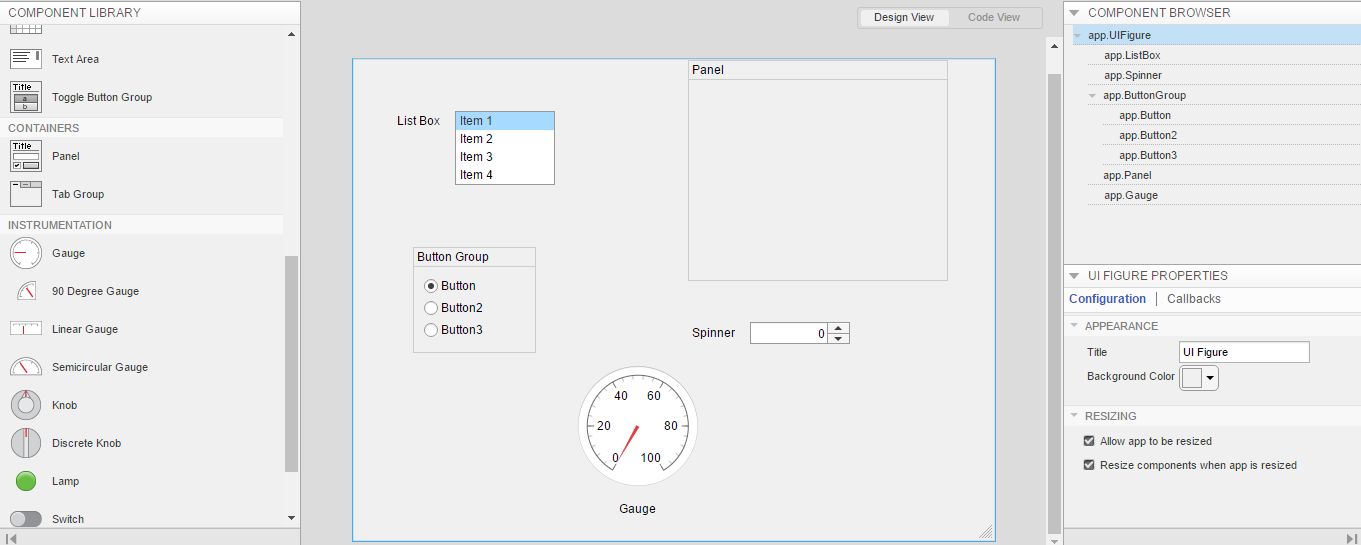
\includegraphics[width=\linewidth]{imagenes/interfaz_appdesigner.PNG}
	\caption{Interfaz de \textit{App Designer}.}
	\label{fig:appdesigner}
\end{figure}

\textit{App Designer} tiene una forma simple de uso: colocar los elementos requeridos en la ventana creada, arrastrándose intuitivamente con el puntero del ordenador. Estos elementos, por lo general, sirven para introducir datos o realizar una acción, como es el caso de los botones. Una vez incorporados todos los elementos deseados, se configura uno o varios botones con la finalidad de que al ser pulsados se realice una acción determinada por el código interno de la figura. En este caso, se diseñaron dos tipos de ventana: una de introducción de datos cuyo único botón procede a la ejecución de la simulación con los datos introducidos, y otra para determinar qué datos de salida se desea que sean representados gráficamente, a través de botones mayormente.

\begin{figure}[h!]
	\centering
    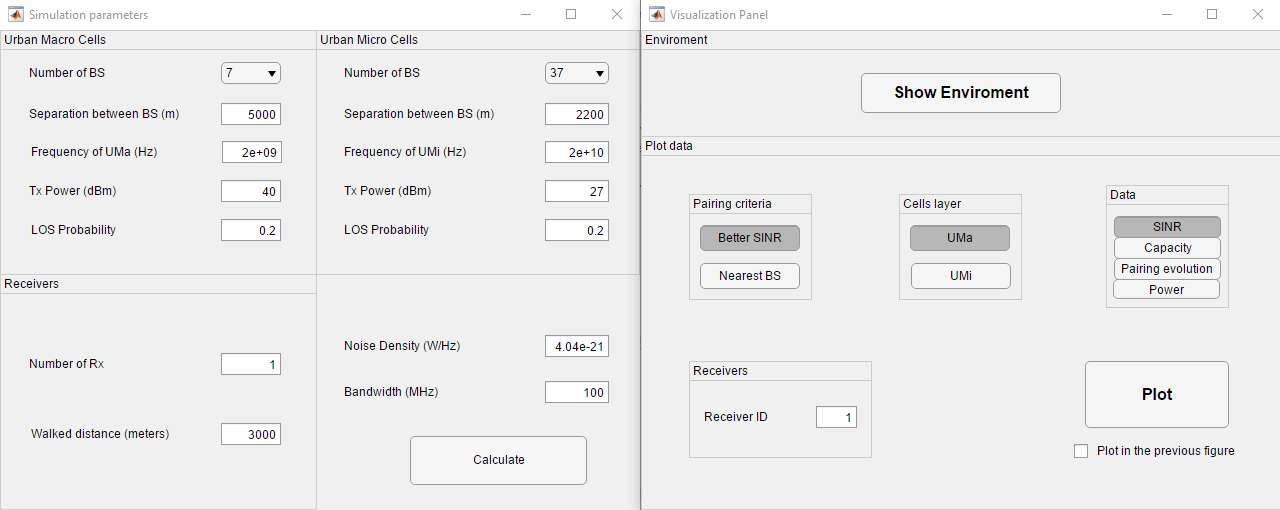
\includegraphics[width=\linewidth]{imagenes/ventanas.PNG}
	\caption{Interfaces gráficas de usuario que constituyen \textit{5Gneralife}.}
	\label{fig:ventanas_graficas}
\end{figure}

La ventana de introducción de datos cuenta con un campo de texto y/o numérico por cada uno de los atributos con los que cuenta la clase \textit{Parameters}. Su función es la de recoger cada uno de ellos y generar un objeto de dicha clase que reúna todos los parámetros deseados. A grandes rasgos, se podría decir que esta ventana implementa una interfaz gráfica del constructor de la clase \textit{Parameters}. Al pulsar el botón dedicado a cerrar la ventana y crear el objeto, se realiza una llamada a dos funciones: al constructor de \textit{Parameters} y a la función que la misma ventana incluye para cerrarse:

\begin{lstlisting}[style=Matlab-editor, basicstyle=\tiny]
            params = Parameters(app.freq_uma.Value, app.freq_umi.Value, str2double( app.number_of_uma.Value ), str2double( app.number_of_umi.Value ),...
                app.dist_between_uma.Value, app.dist_between_umi.Value, app.number_of_rx.Value, app.walked_distance.Value, app.tx_power_uma.Value, ...
                app.tx_power_umi.Value, app.BW.Value, app.No.Value, app.los_uma.Value, app.los_umi.Value);
            
            save('parameters.mat', 'params');
                
            delete(app);
\end{lstlisting}

El intercambio de variables entre el \textit{script} principal de ejecución y el código interno de la ventana se realiza a través del disco duro. La ventana almacena en el directorio principal las variables en forma de fichero para que posteriormente el \textit{script} las recoja y elimine del disco duro.

Por otro lado, en cuanto a la ventana dedicada a representar gráficamente los resultados de salida, cuenta con una constitución distinta ya que se ha concebido para facilitar las representaciones gráficas de las que dispone \textit{5Gneralife}. Esto incluye la disposición geográfica de los elementos -botón \textit{show\_enviroment}- y la representación de los valores de las variables de salida a lo largo de todo el recorrido del usuario seleccionado en \textit{Receiver ID} -SINR, capacidad, potencia, etc.-.

Para ello, al pulsar el botón \textit{Plot} se llama a la función encargada de trazar los datos en una nueva figura, pasando como argumentos las variables necesarias de acuerdo a la selección de los botones de la interfaz por parte del usuario. Esto se ha implementado a través de un \textit{script} incluido en el código interno de la ventana que evalúa el estado de cada uno de los botones seleccionables y realiza la llamada a la función de acuerdo a las opciones seleccionadas por el usuario:

\begin{lstlisting}[style=Matlab-editor, basicstyle=\tiny]
rx_id = app.no_rx.Value;
hold_on = app.holdon.Value;

if (app.uma.Value)
    type = 'UMa';
    pairing = app.pairing_uma;
else
    type = 'UMi';
    pairing = app.pairing_umi;
end

if (app.better_sinr.Value)
    criteria = 'SINR';
else
    criteria = 'Nearest BS';
end

if (app.sinr.Value)
    data = 'SINR';
    if strcmp(type,'UMa')
        input = app.sinr_uma;
    else
        input = app.sinr_umi;
    end
elseif (app.capacity.Value)
    data = 'Capacity';
    if strcmp(type, 'UMa')
        input = app.capacity_uma;
    else
        input = app.capacity_umi;
    end
elseif (app.power.Value)
    data = 'Power';
    if strcmp(type,'UMa')
        input = app.rx_power_uma;
    else
        input = app.rx_power_umi;
    end
else
    data = 'Pairing';
    input = pairing;
end

show_data(criteria, type, data, rx_id, pairing, hold_on, input);
\end{lstlisting}

\section{Documentación y publicación del código}

Puesto que \textit{QuaDRiGa} se encuentra publicado bajo Licencia Pública General Reducida de GNU, conocida por su nombre en inglés GNU \ac{lgpl} con propósitos educativos, se ha decidido seguir con la misma filosofía de publicación y el código del simulador ha sido publicado su propio repositorio en GitHub \cite{publicacion}, con el propósito de ofrecer el uso del simulador a todo aquél que lo desee, o bien, ofrecer la posibilidad de mejorar gracias a las contribuciones que cualquier colaborador puede aportar.

En dicho repositorio se encuentra la documentación HTML de todo el proyecto, con sus especificaciones sobre formas de uso, descripción de variables, comentarios de uso y ejecución, instrucciones... En él también se puede encontrar el código fuente de la presente memoria, escrita en el sistema de escritura de documentos LATEX.

De este modo, se facilita la distribución del código y se abre posibilidad a que el proyecto quede al servicio de la comunidad científica y técnica, dando lugar siempre a que el proyecto crezca.
